\chapter{The New Star}
\label{ch:04}



\begin{center}
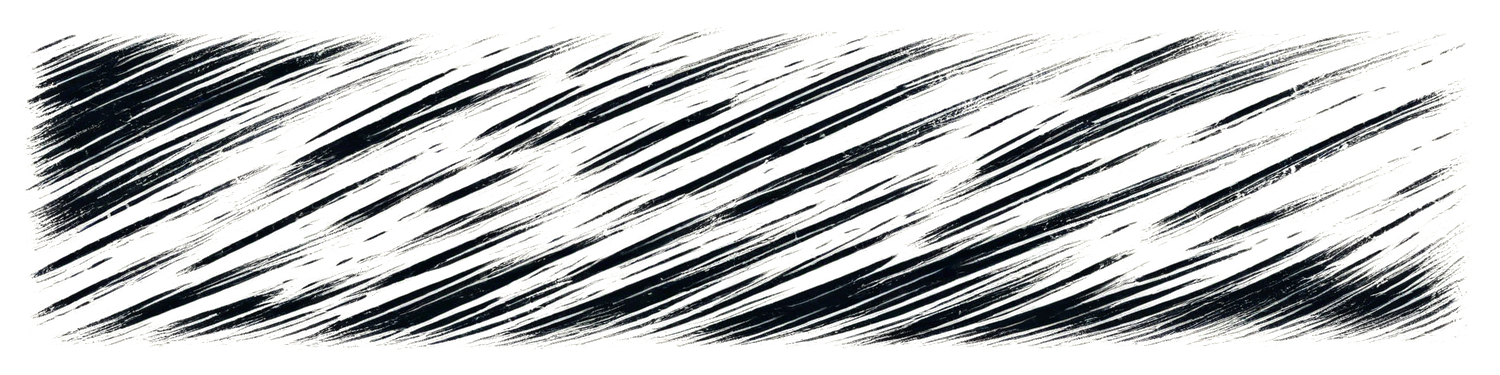
\includegraphics[width=\textwidth]{images/chapterImages/genesis_sketch_00058_.png}
\end{center}

The sky had always contained patterns. Points of light that wheeled through their courses with mathematical precision. Constellations that rose and set according to laws that predated any observation of them. Aurelia had tracked these patterns since she was old enough to tilt her head upward, calculating orbital mechanics before she had context for what orbits were.

She understood the sky the way others understood hunting or territory or the hierarchy of threat. It was simply knowledge that existed in her, built perhaps from observation or perhaps from something deeper—inherited awareness passed down through generations, each adding their calculations to some collective

understanding that had no mechanism of transmission but existed anyway.

And then the sky changed.

She woke that morning to the knowledge before she even opened her eyes. Something was different. The sensation was immediate and undeniable, like waking to find a fundamental constant of physics had shifted. Gravity pulling sideways. Light moving slower. The wrongness of it absolute.

She emerged from the hollow before dawn. The young ones still slept. At the ravine's edge, the other one was already standing, head tilted up at precisely the angle she would have chosen herself. He had felt it too.

They stood separated by twenty body lengths, both staring at the same point in the pre-dawn sky. Waiting for it to become visible. Knowing it would be there. Knowing it would be wrong.

The stars emerged as the last ambient light faded. Familiar patterns resolved themselves—the hunter constellation, the spiral, the twins. Everything in its expected position.

And then, between the familiar patterns, in a space that should have been empty, a new point of light appeared.

Not sudden. It had been becoming visible for several moments, gradual as all starlight is gradual when emerging from twilight. But once visible, it was unmistakable. Brighter than it should be. In a position that violated the expected configuration.

Wrong.

Aurelia's entire body went rigid.

Across the ravine, the other one went equally still.

And everywhere—across the entire continent, across regions she had never seen and would never see—every member of her kind stopped whatever they were doing and froze.

The massive long-necks halted mid-step, their tiny brains nevertheless capable of recognizing celestial anomaly. The swift runners paused in their evening hunt, small mammals forgotten. The armored ones ceased their browsing and lifted their heavy heads to the sky.

And all the small ones, the thinkers, the calculators—every single one of them locked into absolute stillness. From the Builder at his stone formations to the Carver clinging to her cliff face to the Pair in their marsh clearing, every individual capable of complex thought stopped moving.

Even the young ones. Aurelia's three hatchlings emerged from the hollow, drawn by some instinct they were too juvenile to understand. They saw her stillness and mimicked it, their small heads tilting at the same angle as hers, looking at a star they couldn't possibly comprehend the significance of.

For three days, the world held its breath.

\scenebreak

Aurelia didn't move from her position at the ravine's edge. Didn't eat. Barely breathed. The young ones, unable to maintain such stillness, eventually wandered back to the hollow and slept, woke, grew hungry, made their demanding chirps. She didn't respond. They found cached food on their own and ate it messily, uncertain but surviving.

The other one brought more food for them. Placed it where they would find it. Returned to his own position of stillness. They were all still calculating.

Birds continued their patterns. Small mammals scurried through undergrowth. Insects droned. The river flowed. The world continued around them while they remained frozen.

To an observer, it might have looked like mass paralysis. A plague of stillness. Some disease that locked bodies in place while minds remained aware and trapped.

But their minds weren't trapped. Their minds were working at capacity beyond anything evolution had designed for. Processing observational data, running trajectory simulations, calculating mass and velocity and the curved paths objects follow through space. Each individual worked on the problem from their own perspective, their own accumulated knowledge.

Behind the Watcher's eyes, numbers cascaded. She tracked the new star's position against the background of the familiar sky. Measured its movement—minuscule over hours, measurable over days. Extrapolated its path backward, forward. Found the curve it was following.

It wasn't a star. Stars didn't move like this. Stars were fixed points, or moved with such agonizing slowness that their motion only became apparent across generations. This moved with purpose, with directed velocity. This was smaller. Closer.

Much closer than it should be.

Her calculations built on themselves. If it maintained this trajectory, if its velocity held constant (and why wouldn't it?), if her measurements of parallax were accurate (and they were, she'd checked them seventeen times), then...

Then it was coming here.

Not toward the sky—INTO the sky. Into the space this planet occupied. Intersection of orbital paths. Collision course.

The timeline resolved itself through iterative refinement. Each hour of observation added precision. First cycle: sometime in the next decade. Second cycle: within eight years. Third cycle: within seven. Fourth cycle: six years and approximately three seasons.

By the end of the third day, her calculations had stabilized. 2,247 rotations plus or minus twelve. The margin of error was acceptable. The certainty was not.

Around her, the forest had grown quieter. Predators still hunted but with less energy, as if the stillness of so many prey species had robbed hunting of its urgency. Plants continued their patient growth. But the absence of movement from so many thinking creatures created a silence that was almost physical.

On the third evening, as the wrongstar rose again (brighter, always brighter), the calculation completed.

She didn't know how she knew the others had reached the same conclusion. There was no signal. No communication passed between her and the distant Builder or the ancient Carver or the Pair in their marsh. But in the same moment—not similar moments, not roughly the same time, but the SAME instant—every calculating mind on the continent reached identical certainty.

Impact in 2,247 rotations.

Margin of error: negligible.

Options: limited.

Outcome: inevitable.

The stillness broke.

Aurelia's head lowered. Her breathing deepened. Her legs trembled with the exhaustion of three days' stillness. She took one step, then another, moving slowly at first as circulation returned to full function.

Behind her, the young ones emerged from the hollow again, sensing the change. They tumbled toward her with relieved chirps, pressing against her legs. She bent her head to acknowledge them briefly. They were hungry. They would need proper hunting soon, not just cached scraps.

Across the ravine, the other one shook himself—a full-body shiver that ruffled his feathers and reset his stance. He looked toward her for the first time in three days. She looked back.

Neither of them needed to communicate what they now knew. They both carried the same calculation, arrived at through separate processing but identical in conclusion. The knowledge sat between them like a physical object.

2,247 rotations.

He moved first, climbing down into the ravine and then up the other side toward her territory. She didn't signal retreat or warning. The boundaries that had existed three days ago felt less important now. Less real.

He approached to within three body lengths—closer than they'd been before. Close enough that she could see the pattern of his feathers clearly, the small scar on his snout from some old injury, the amber intensity of his eyes.

The young ones watched him warily but didn't flee. They had been eating food he provided for three days. That created some basic trust, even in juvenile minds that understood little else.

He stood there for a long moment. Then he turned so he was beside her rather than facing her. Both of them looking in the same direction. And together, they looked up as the last light faded and the stars emerged.

The wrongstar appeared right where it should, where the mathematics said it must. Brighter than three days ago. Still approaching.

Their tails hung parallel, separated by less than a body width. When a breeze moved through the ravine, the feathers at the tips touched. Just barely. Just enough.

She didn't move away from the contact.

They stood that way until full dark, until the temperature dropped and the young ones retreated to the hollow for warmth. Then, without discussion or signal, they both moved.

Not to roost. Not to hunt. To work.

The pattern she had created—the three stones in their precise geometry—was a beginning. Only a beginning. The calculations in her head required external representation, some way to process complexity beyond what even her enhanced cognition could hold simultaneously.

She began moving stones, expanding the pattern. Large ones that required effort to shift. Small ones for fine detail. Arrangements that would mean nothing to most creatures but that encoded information for those who could read it.

The other one watched for several minutes, understanding flowing without explanation. Then he began gathering stones himself, placing them in positions that supported her pattern. His mathematics weren't as sophisticated as hers—she could sense that in the choices he made, the slight suboptimality of some placements. But he grasped the fundamental structure. Could see what she was building.

They worked through the night. Not speaking. Not touching except when they reached for the same stone and their hands brushed. Then they would pause for half a heartbeat before one yielded and took a different stone.

The young ones slept. The river flowed. Above, the stars wheeled on their appointed courses, and among them, the wrongstar traced its patient arc toward intersection.

By dawn, the pattern had tripled in size. The original three stones now marked one corner of something larger, more complex. A timeline beginning to take shape. A calculation rendered in stone and space and geometric relationship.

It wasn't finished. Wouldn't be finished for seasons. But it had grown from concept to physical form. From thought to matter.

As the sun cleared the treeline, the other one finally moved toward his own roosting site. Exhausted. But he didn't return to wherever his original territory was. He found a hollow in a tree twenty body lengths from hers and settled into it.

Close enough to help. Close enough to contribute. Close enough to matter.

Aurelia returned to her own hollow, where the young ones were waking, hungry and demanding. She led them to hunt, teaching them the precision their developing minds could handle, saving the deeper calculations for later.

When later would come was now quantified. 2,247 rotations. Every one of them would count.

Above, visible even in daylight if one knew where to look, the wrongstar continued its approach. Gravity and momentum and the ancient mathematics of orbits, all converging toward a single point in time.

Inevitable.

Unless.

The thought formed in her mind not as words but as pure mathematics. A probability function. A chance measured in percentages that would have seemed impossibly small to a human mathematician.

But not zero.

Not quite zero.

And so the work continued.

